% Chapter Template

\chapter{Correct by Construction (CbyC) } % Main chapter title

\label{Chapter_CbyC} % Change X to a consecutive number; for referencing this chapter elsewhere, use \ref{ChapterX}

%----------------------------------------------------------------------------------------
\section{Overview}

The CbyC software development methodology proposes to limit software 
defects by:  
\begin{enumerate}
	\item making it difficult to introduce errors, and
	\item detecting and removing errors as early as possible.
\end{enumerate}

CbyC technique emphasises the use of mathematically rigorous tools. CbyC proposes
using mathematical formal language to define the specification and high-level design
of a system. This provides a precise description of the system's behaviour and a
precise model of its characteristics. Using a mathematical language also allows
the use of automated tools to verify the specification and design \parencite{CbyCMan}.

CbyC code is designed around information flow. The information flow is
defined using a contract-based notation. The contract-based notation is
used to define the abstract state of the program and the information relationships
across boundaries. CbyC proposes using programming languages and tools that allow
for the code and contracts to be validated using static analysis \parencite{CbyCMan}.
 
%----------------------------------------------------------------------------------------

\section{Correct by Construction Process}\label{CbyCDevWorkflow}

The CbyC process is described in terms of the artefacts it produces (Figure \ref{fig:CbyCDev}): 

\begin{itemize}
	\item System requirements specification;
	\item Formal specification;
	\item Formal design;
	\item System test specification;
	\item INFORMED design;
	\item Code;
\end{itemize}

Using the CbyC process every process artefact can be validated.The semantic gap 
between process artefacts are kept small. This makes it possible to show that later 
process artefacts conform to earlier process artefacts \parencite{Tokeneer}.

We now describe each artefact and how it is created.

\begin{figure}[H]
	\centering
	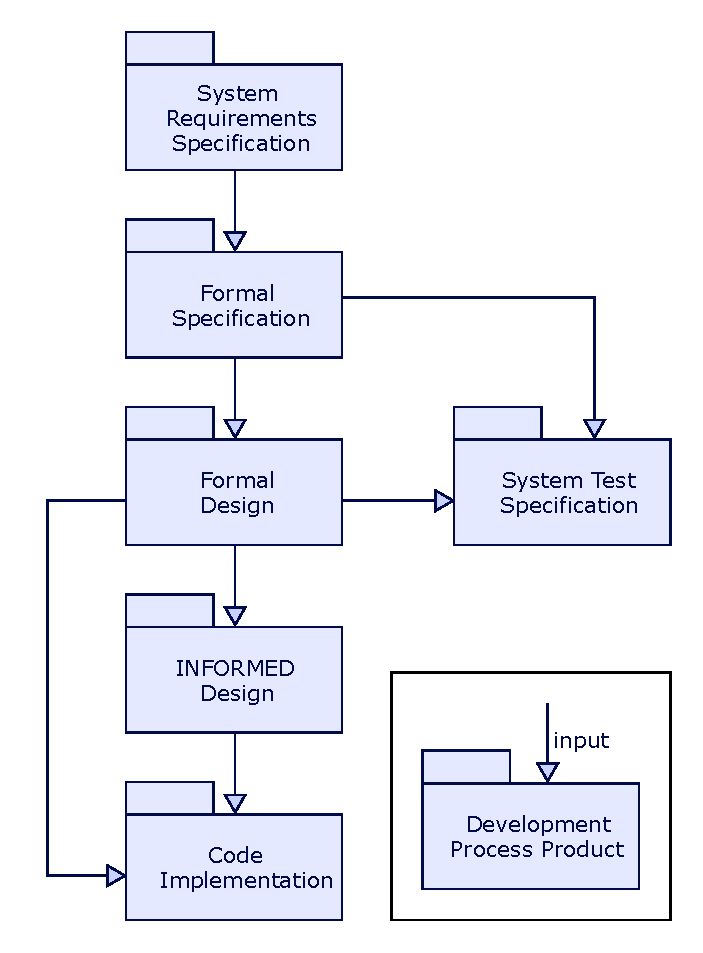
\includegraphics[scale=0.75]{Figures/CbyC_process.pdf}
	\decoRule
	\caption{CbyC process artefacts.}
	\label{fig:CbyCDev}
\end{figure}

\subsection{System Requirements Specification}

The requirements analysis identifies the needs of the stakeholders, the desired 
behaviour of the system, and any non-behavioural system characteristics \parencite{Tokeneer}. 

Requirements management extends throughout the system's development, but it is 
most significant at the beginning, where it is used to identify \parencite{Tokeneer}:
\begin{itemize}
	\item the stakeholders, who have an interest in the development and use of the system;
	\item the system boundary, to clarify the scope of the project and the interfaces to external systems;
	\item the expected use, in terms of interactions between users and the system;
	\item system properties, such as security properties, performance properties, etc.
\end{itemize}

Each requirement should be traceable through every process artefact \parencite{Tokeneer}.
The requirements are compiled into the System Requirements Specification document.

The System Requirements Specification is created to \parencite{Tokeneer}:
\begin{itemize}
	\item early in the project clarify the system's boundary (what is in scope 
		and what is out of scope, and the necessary interfaces to external systems);
	\item agree on the system requirements with all of the stakeholders;
	\item document the requirements with enough procession so that the Formal 
		Specification can be developed with minimal customer input;
	\item clarify and document the assumptions about the behaviour the environment
		external to the system being developed;
	\item identify and manage conflicting expectations between stakeholders.
\end{itemize}

\subsection{Formal Specification}

The aim of the Formal Specification is to unambiguously describe what the system
will do. This is to help the developer and the client gain a common understanding
of the system \parencite{Tokeneer}.

The level of abstraction is important. The Formal Specification should not describe 
the system's implemented. Internal details are deliberately left very abstract. 
Interactions with the external environment are specified, but may also be abstract \parencite{Tokeneer}.

The Formal Specification is written in mathematical notation with an English 
narrative. The specification is divided into small components that can be reasoned
about individually. The small components are then combined to describe the system
as a whole \parencite{Tokeneer}.

The Formal Specification is created because it \parencite{Tokeneer}:
\begin{itemize}
	\item provides an unambiguous description of what the system does. This is
		important for gaining client approval of the system's behaviour.
	\item can be shown to be complete.
	\item can be formal verified, i.e. it can be proved consistent.
\end{itemize}

\subsection{Formal Design}

The aim of the formal design is to elaborate the abstract aspects of the Formal 
Specification to explain how the system will be implemented. The Formal Design 
describes the system in terms of concrete state and operations using types that
are easily implemented. The Formal Design is the source of the required functional
behaviour used during implementation  \parencite{Tokeneer}.

The design is written in the same mathematical notation as the Formal Specification.
This means that the design can be formally verified and errors can be uncovered
before implementation starts \parencite{Tokeneer}.

The reasons for producing a Formal Design are  \parencite{Tokeneer}:
\begin{itemize}
	\item It provides an unambiguous description of how the system does what the formal specification requires.
	\item It can be shown to be complete.
	\item It can be formal verified, i.e. it can be proved consistent.
\end{itemize}

\subsection{System Test Specification}

The aim of the System Test it to demonstrate that the system has the correct 
behaviour as specified in the Formal Specification. This differs from the goals of
acceptance testing which is designed to demonstrate that the System meets
its requirements. System Testing aims to achieve 100\% coverage of the formal 
specification. Thus so all possible behaviours described in the formal specification
should be exercised at least once \parencite{Tokeneer}.

The Formal Design is a refinement of the Formal Specification. Therefore the Test
Specification can also be written against the Formal Design if you want to tests 
details of the design \parencite{Tokeneer}.

All System tests are specified in a System Test Specification prior to their 
execution.  The tests are specified as scenarios that might occur in typical usage
of the system. The specification includes documentation of the expected outcome
of the test. System test specifications also traces each test to the components
of the Formal Specification/Design that the test attempts to exercise \parencite{Tokeneer}.

Where code coverage metrics need to be captured, this is be done during the
System test. This allows us to question the use of any code that cannot be covered
by a system test. If the code is valid then focused unit tests should be added to
cover the code \parencite{Tokeneer}.

The reasons for producing a System Test Specification are \parencite{Tokeneer}:
\begin{itemize}
	\item A system test focuses on testing the behaviour of the whole system against
		the expected (specified) behaviour.
	\item A system test is likely to find faults caused by the incorrect interaction
		of modules within the system.
	\item System testing complements static analysis, in that it confirms the 
		dynamic behaviour.
\end{itemize}

\subsection{INFORMED Design}
CbyC design methodology is based on information flow. The information flow is 
defined using a contract-based notation. The contract-based notation is used to
define the abstract state of the program and the information relationships across
boundaries \parencite{CbyCMan}.

Consideration of information flows at the design stage leads to programs with the
desirable properties of abstraction, encapsulation, high cohesion and loose 
coupling \parencite{Tokeneer}.

The \textbf{IN}formation \textbf{F}low \textbf{OR}iented \textbf{ME}thod of
object \textbf{D}esign (INFORMED) design provided an architectural framework
in which to perform the implementation. Consideration of information flows at the
design stage results in programs with the desirable properties of abstraction, 
encapsulation, high cohesion and loose coupling \parencite{Tokeneer}.

The INFORMED design aids maintenance and upgrades of the software by providing a
route-map from the Formal Design to the code \parencite{Tokeneer}.

The reasons for producing an INFORMED Design are \parencite{Tokeneer}:
\begin{itemize}
	\item It focuses on the system architecture and ensures that the architecture 
		fits the information flow model.
	\item It provides the mapping from the Formal Design to the Code before writing
		the code.
	\item It complements the Formal Design without duplicating functional information.
\end{itemize}

\subsection{Code Implementation}
We start by writing the module specification. The specification is the public 
interface and the contracts governing the global state of the module. The contacts
specify how inputs are allowed to influence outputs \parencite{Tokeneer}. 

After writing the specification we implement the module body. The Formal Design is
detailed enough to make that the mapping from the design to the code simple 
\parencite{Tokeneer}.

Modules providing infrastructure are developed early. Module are implementation 
in a order that allows system level functionality to be added incrementally. This
means that a basic system can be built as soon as possible and functionality is 
added in subsequent builds. This has the advantage of addressing code integration
risks as early as possible \parencite{Tokeneer}.

By using languages that allows static analysis we can evaluate the code 
contracts at build time. Thus if the code builds it is correct as specified by the
contracts \parencite{Tokeneer}.